\documentclass[11pt]{amsart}

% Margins
\usepackage[headheight=65pt]{geometry}
\geometry{
  top=1 in,
  inner=1 in,
  outer=1 in,
  bottom=1 in,
  headheight=3ex,
  headsep=2ex,
}

% Personal info, class, assignment
\def \fnamea{Dennis}
\def \fnameb{Neill}
\def \lnamea{Windham}
\def \lnameb{Shikada}
\def \class{CSCI 5448}
\def \hwnum{5} % Homework number
\def \assgn{Project \hwnum}
\newif\ifcode % Switch to toggle Python code insertion, see the end of the document for the value assignment

% Header
\usepackage{fancyhdr}
\pagestyle{fancy}
\lhead{\lnameb\ \& \lnamea}
\fancyfoot{}
\chead{\assgn}
\rhead{Page \thepage}
\renewcommand{\headrulewidth}{2pt}
%\renewcommand{\footrulewidth}{1pt}
\usepackage{pdflscape}


\usepackage{enumitem}
\usepackage{tabularx}
\usepackage{amssymb,amsmath,amsthm,amscd,mathrsfs,graphicx,color,pdfpages}
\usepackage[cmtip,all,matrix,arrow,tips,curve]{xy}
\usepackage[active]{srcltx}
\usepackage{mathpazo}
\usepackage{setspace}\doublespacing 
%Double space, and make it easier for the grader to grade your homework.
\usepackage{hyperref}
\usepackage[usenames,dvipsnames]{xcolor}
\usepackage[style=science,sortcites=true,sorting=nyt,backend=biber]{biblatex}
\hypersetup{colorlinks=true,citecolor=ForestGreen,linkcolor=Maroon,urlcolor=NavyBlue}

% Python raw code insertion
\usepackage{listings}
\usepackage{color}

% Python linting settings
\definecolor{dkgreen}{rgb}{0,0.6,0}
\definecolor{gray}{rgb}{0.5,0.5,0.5}
\definecolor{mauve}{rgb}{0.58,0,0.82}
\lstset{frame=tb,
  language=Python,
  aboveskip=3mm,
  belowskip=3mm,
  showstringspaces=false,
  columns=flexible,
  basicstyle={\small\ttfamily},
  numbers=none,
  numberstyle=\tiny\color{gray},
  keywordstyle=\color{blue},
  commentstyle=\color{dkgreen},
  stringstyle=\color{mauve},
  breaklines=true,
  breakatwhitespace=true,
  tabsize=3
}

% References
\addbibresource{./references.bib}

% Allows vertical lines in matrices like in tables
% Usage:
% \begin{bmatrix}[cc|cc] ...
\makeatletter
\renewcommand*\env@matrix[1][*\c@MaxMatrixCols c]{%
  \hskip -\arraycolsep
  \let\@ifnextchar\new@ifnextchar
  \array{#1}}
\makeatother

\newcommand{\marg}[1]{\normalsize{{\color{blue}\footnote{{\color{blue}#1}}}{\marginpar[\vskip -.3cm {\color{blue}\hfill\thefootnote$\implies$}]{\vskip -.3cm{ \color{blue}$\impliedby$\thefootnote}}}}}

\newcommand{\qc}[1]{\marg{#1}}

\setlength\fboxsep{.3cm}
\setlength\fboxrule{.05cm}

% Custom boxes
\newcommand*{\boxedcolor}{orange}
\makeatletter
\renewcommand{\boxed}[1]{\textcolor{\boxedcolor}{%
  \fbox{\normalcolor\m@th$\displaystyle#1$}}}
\makeatother

\makeatletter
\newcommand{\boxedred}[1]{\textcolor{red}{%
  \fbox{\normalcolor\m@th$\displaystyle#1$}}}
\makeatother

\makeatletter
\newcommand{\boxedblue}[1]{\textcolor{blue}{%
  \fbox{\normalcolor\m@th$\displaystyle#1$}}}
\makeatother

% Begin Document
\begin{document}

%region Author, Title, Abstract, TOC
\author[\lnamea]{\fnamea\ \lnamea\\\fnameb\ \lnameb}
\date{\today}
\title[\assgn]{\assgn \\ \ \\\class}
\maketitle
\tableofcontents
%endregion

\newpage
\section*{\textbf{Project Summary}}
\subsection*{Title}
\begin{center}
    \textit{Object Oriented Civilization Game Clone}
\end{center}

\subsection*{Team Members} \phantom{}

\begin{table}[htbp]
    \begin{tabularx}{\textwidth}{l|l|l}
        \textbf{Name}    & \textbf{Role} & \textbf{Email} \\
        \hline
        Neill Shikada    & Graduate Student & Neill.Shikada@colorado.edu
        \\
        Dennis Windham   & Graduate Student & dene5275@colorado.edu  \\
        Bruce Montgomery & Instructor & bruce.r.montgomery@colorado.edu 
    \end{tabularx}
\end{table}

\subsection*{Overview} \phantom{}

Our project is a small Unity Engine video game based on Sid Meier's Civilization. Our version of the game will be based on a square game board as opposed to Civilization's hexagonal board. There will be one human player and several AIs. Each player will have a starting city that can generate one of three rock-paper-scissors-like unit types every 3 turns, and control their movement in the game board. Units and cities have individual health bars and attack strengths, depletion of the health bar leads to removal of the respective entity from the game. A player loses when their city is removed from the game, and the last remaining player wins.

\newpage
\subsection*{Project Requirements} \phantom{}
\begin{itemize}
    \item System Requirements
    \begin{itemize}
        \item The game needs to be fully portable across two major desktop operating systems: Windows (10+) and Linux (kernel 5.15+).
        \item Hardware requirements need to be modest, not exceeding the capabilities of entry-level consumer chips.
    \end{itemize}
    \item Game Board
    \begin{itemize}
        \item The game board needs to be a square grid of a size that facilitates good gameplay for 2-3 players, likely between $20 \times 20$ and $30 \times 30$.
        \item The game board needs to be able to fit the entire game screen as we do not intend to support camera controls.
        \item The game board needs to be interactive to the human user: they will be able to use their mouse to select a unit, get a prompt for which cells the unit may move into, and move the unit by selecting an available cell.
        \item No two units should be able to share the same cell in the game board.
    \end{itemize}
    \item Gameplay
    \begin{itemize}
        \item Players take turns sequentially. Each turn, the player can use all of their units once, choosing to either move or attack, and produce a new unit at the City. The player needs to be able to skip the turn if they are happy with their decisions and do not to finish the turn.
        \item By default, each player has one starting city that can create a unit every 3 turns. The starting city has its own attack power, meaning that units that siege it take damage. A city has $500$ base HP.
        \item The human player must be able to select one of three base civilization types that determine gameplay changes:
        \begin{itemize}
            \item Conquerors
            \begin{itemize}
                \item Damage dealt to enemy cities is increased by $\times 1.5$.
                \item Civilization's own city has $25\%$ less health.
            \end{itemize}
            \item Barbarians
            \begin{itemize}
                \item City can produce units every $2$ turns instead of $3$.
                \item Every unit has $30\%$ less health.
            \end{itemize}
            \item Defenders
            \begin{itemize}
                \item City has $\times 2$ health and attack power.
                \item City can produce units every $4$ turns instead of $3$.
            \end{itemize}
        \end{itemize}

        \item There will be $3$ unit types available to every player. To attack, a unit always needs to be in a cell adjacent to their target. Every unit has the base attack damage of $30$ and a total of $100$ HP.
        \begin{itemize}
            \item Melee
            \begin{itemize}
                \item Deals $\times 1.5$ damage to Ranged units.
                \item Deals $\times 0.5$ damage to Airborne units.
            \end{itemize}
            \item Ranged
            \begin{itemize}
                \item Deals $\times 1.5$ damage to Airborne units.
                \item Deals $\times 0.5$ damage to Melee units.
            \end{itemize}
            \item Airborne
            \begin{itemize}
                \item Deals $\times 1.5$ damage to Melee units.
                \item Deals $\times 0.5$ damage to Ranged units.
            \end{itemize}
        \end{itemize}
        \item When a city or a unit lose all their HP, they are removed from the game. If a city is removed, the player who owns the city instantly loses and all their units are removed from the game. If the human player loses, the game is over.
        \item Total damage done by units of each player needs to be tracked and displayed at the end of the game.
        \item The player may choose to quit the game early, at which point they automatically lose and the game concludes.
    \end{itemize}
    \item AI
    \begin{itemize}
        \item The game needs to have a basic AI for the human player to play against. 
        \item The AI will follow simple heuristics:
        \begin{itemize}
            \item Keep unit type split close to $1:1:1$ when producing new units.
            \item For every available unit, take the greedy action: if there is a nearby enemy unit or a city, attack them, if not, move towards the closest enemy city.
        \end{itemize}
    \end{itemize}
    \item UI
    \begin{itemize}
        \item The UI needs to initially display a civilization type choice to the player, along with respective bonuses.
        \item During the actual gameplay the UI needs to communicate to the player when they may produce new units.
        \item The UI needs to tell the player what units may be selected, and what their available actions are after selection.
        \item After the game is over, the human player will be presented with a scoreboard showing whether they won or lost, and how much damage their units have done in total.
        \item The player needs to have an button to quit the running game.
    \end{itemize}
\end{itemize}

\newpage
\subsection*{Users and Tasks: Use Cases} \phantom{}
The system will have a single human user. See Figure \ref{fig:use_cases} for the Use Case diagram.
\begin{figure}[h!]
    \begin{center}
    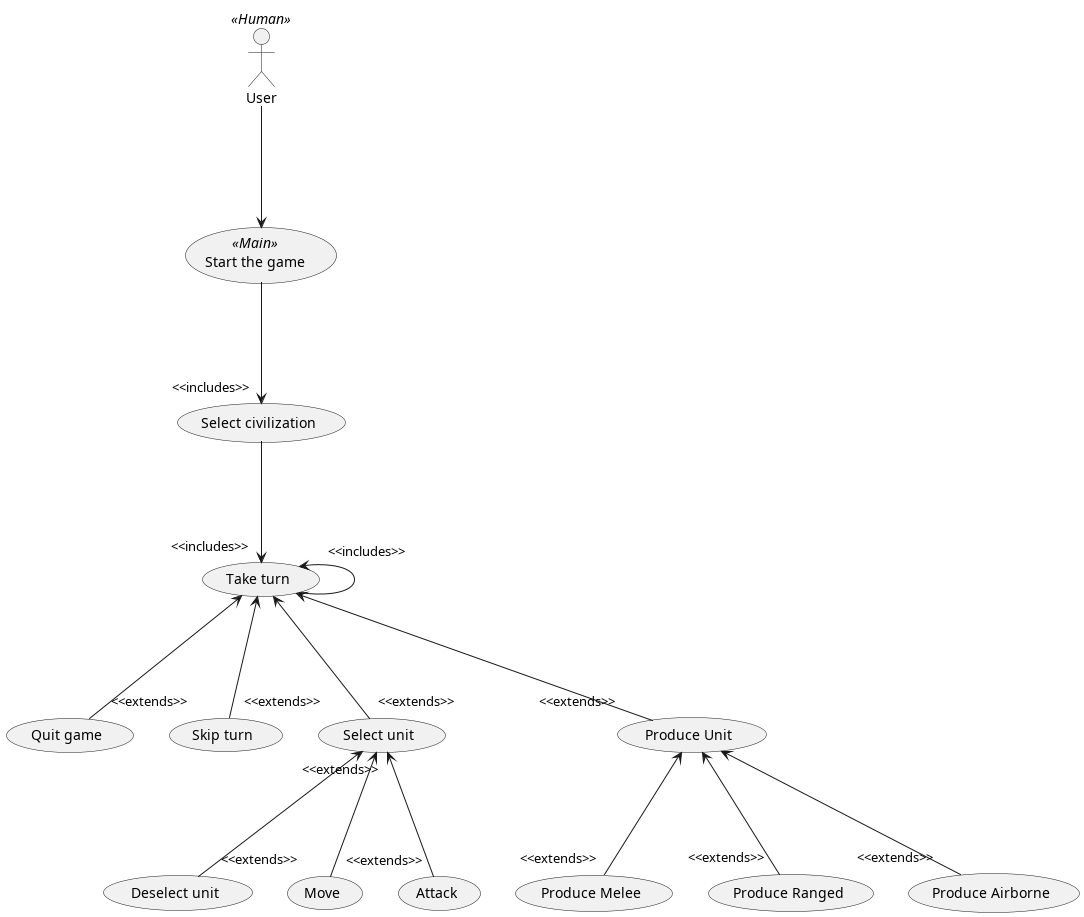
\includegraphics[height=160mm]{../diagrams/use_cases/use_cases.png} \\
    \caption{Use case diagram.}
    \label{fig:use_cases}
    \end{center}
\end{figure}

\newpage
\subsection*{UML Activity or State Diagram (N)} \phantom{}
\subsection*{Architecture Diagram (N)} \phantom{}
\subsection*{Data Storage} \phantom{}

The game will keep track of its state in memory. After the an ending condition is reached, the game will save some statistics to a text file:
\begin{itemize}
    \item Turns taken to finish the game.
    \item Endgame condition for the human player.
    \item Total damage done by each player's units.
    \item How many units of each type were created throughout the game by each player.
\end{itemize}

\subsection*{UI Mockups / Sketches (N)} \phantom{}
\subsection*{UML Class Diagram \& Pattern Use (D)} \phantom{}
\subsection*{User Interactions / UML Sequence Diagrams (N)} \phantom{}


%\codetrue % Uncomment to enable code insertion
\ifcode
    % Python code section, toggled by the switch above
    % The code file is expected to be follow the "hw{\hwnum}.py" naming convention
    \newpage
    \section*{Code}
    \label{sec:code}
    \lstinputlisting[language=Python]{Code/hw\hwnum.py}
\fi


% \includepdf[scale=0.98, pagecommand={\section*{Appendix A: Class Diagram for RotLA}\pagestyle{fancy}}\label{sec:appendixa}]{../uml/game_diagram.png}


\end{document}
